\documentclass[10pt, aspectratio=169]{beamer}

% --- Theme and Visuals ---
\usetheme{metropolis} % Clean, modern theme
\setbeamercolor{background canvas}{bg=white}
\setbeamercolor{palette primary}{bg=darkgray, fg=white}

% --- Packages ---
\usepackage[utf8]{inputenc}
\usepackage[T1]{fontenc}
\usepackage{amsmath, amssymb, amsfonts}
\usepackage{graphicx}
\usepackage{booktabs}
\usepackage{tikz}
\usetikzlibrary{arrows.meta, positioning, shapes.geometric}

% --- Custom Commands/Styles ---
\definecolor{mainblue}{RGB}{0, 102, 204}
\definecolor{highlight}{RGB}{204, 0, 0}

% --- Title Information ---
\title{MN-BO v3.2: Snowball Multi-View Search Architecture}
\subtitle{Optimizing Complex Landscapes via Ordered Operator Chains}
\author{Antigravity Research Team}
\date{\today}

\begin{document}

% --- Title Slide ---
\begin{frame}
    \titlepage
\end{frame}

% --- Section 1: Business Flow ---
\section{Workflow v3.2: The Snowball Search}

\begin{frame}{System Architecture: Snowball Mechanism}
    \begin{columns}
        \begin{column}{0.6\textwidth}
            \textbf{Core Logic: Data Persistence}
            \begin{itemize}
                \item \textbf{Initialization}: 5 random points in target space.
                \item \textbf{Outer Loop ($M$ rounds)}: 
                \begin{itemize}
                    \item Meta-GP suggests 8D transformation parameters.
                \end{itemize}
                \item \textbf{Inner Loop ($N$ steps)}: 
                \begin{itemize}
                    \item Standard BO exploration in the warped space.
                \end{itemize}
                \item \textbf{Snowballing}: Data is \textit{never reset}. Each new perspective inherits all previous observations.
            \end{itemize}
        \end{column}
        \begin{column}{0.4\textwidth}
            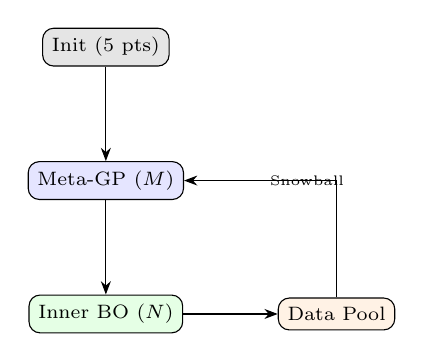
\begin{tikzpicture}[node distance=1.2cm, auto, >=Stealth]
                \node[draw, rounded corners, fill=gray!20] (init) {\scriptsize Init (5 pts)};
                \node[draw, rounded corners, fill=blue!10, below=of init] (meta) {\scriptsize Meta-GP ($M$)};
                \node[draw, rounded corners, fill=green!10, below=of meta] (bo) {\scriptsize Inner BO ($N$)};
                \node[draw, rounded corners, fill=orange!10, right=of bo] (pool) {\scriptsize Data Pool};
                
                \draw[->] (init) -- (meta);
                \draw[->] (meta) -- (bo);
                \draw[->] (bo) -- (pool);
                \draw[->] (pool.north) |- (meta.east) node[near end, right] {\tiny Snowball};
            \end{tikzpicture}
            \vspace{0.5cm}
            \centering
            \textbf{Total Budget: 120 Steps}
        \end{column}
    \end{columns}
\end{frame}

% --- Section 2: Logic Core ---
\section{The Ordered Operator Chain}

\begin{frame}{From Discrete Permutations to Continuous Intensity}
    \textbf{Problem}: How to combine multiple geometric transformations?
    \textbf{Solution}: A strictly ordered execution pipeline where parameters control ``intensity''.
    
    \vspace{0.5cm}
    \begin{center}
    \begin{tikzpicture}[node distance=0.3cm, auto, >=Stealth]
        \node[draw, rectangle, fill=blue!5] (log) {\scriptsize 1. LogWarper};
        \node[draw, rectangle, fill=blue!10, right=of log] (pow) {\scriptsize 2. PowerWarper};
        \node[draw, rectangle, fill=blue!15, right=of pow] (ali) {\scriptsize 3. Aligner};
        \node[draw, rectangle, fill=blue!20, right=of ali) (sca) {\scriptsize 4. Scaler};
        
        \draw[->, thick] (log) -- (pow);
        \draw[->, thick] (pow) -- (ali);
        \draw[->, thick] (ali) -- (sca);
    \end{tikzpicture}
    \end{center}
    
    \begin{itemize}
        \item \textbf{Ordered Sequence}: Ensures numerical stability and mathematical consistency.
        \item \textbf{Intensity Control}: Discrete ``yes/no'' for an operator is replaced by a continuous parameter (e.g., power factor $\alpha$, log threshold $\lambda$).
    \end{itemize}
\end{frame}

% --- Section 3: MN Configuration ---
\section{Strategic $M/N$ Balancing}

\begin{frame}{Breadth vs. Depth: The $M/N$ Trade-off}
    The performance of MN-BO is governed by the ratio of \textbf{Perspectives ($M$)} to \textbf{Exploration ($N$)}.
    
    \begin{itemize}
        \item \textbf{Low $M$, High $N$}: ``Deep Drilling'' - prone to getting stuck in local optima if the initial perspective is poor.
        \item \textbf{High $M$, Low $N$}: ``Surface Skimming'' - fails to refine the search because the GP model never matures in any single space.
        \item \textbf{Robust Sweet Spot}: Current findings suggest $(M=8, N=12)$ as a strong general-purpose starting point.
    \end{itemize}
    
    \begin{block}{Insight}
        Extremely small $M$ (cannot learn meta-patterns) or extremely small $N$ (cannot exploit local gradients) are logically unsustainable.
    \end{block}
\end{frame}

% --- Section 4: Function-Specific Adaptation ---
\section{Landscape Specificity}

\begin{frame}{Function-Specific $M/N$ Adaptation}
    There is no ``Free Lunch''. Optimal configuration depends on the \textbf{Objective Landscape}.
    
    \begin{columns}
        \begin{column}{0.5\textwidth}
            \centering
            \textbf{Needle Type (针尖型)}
            \begin{itemize}
                \item Sharp, narrow optima.
                \item High $N$ (Depth) is critical to ``fall into'' and refine the peak.
            \end{itemize}
        \end{column}
        \begin{column}{0.5\textwidth}
            \centering
            \textbf{Plateau Type (平原型)}
            \begin{itemize}
                \item Vanishing gradients, large flat areas.
                \item High $M$ (Perspectives) is critical to find any signal.
            \end{itemize}
        \end{column}
    \end{columns}
    
    \vspace{0.4cm}
    \textbf{Future Direction}: \textit{Adaptive MN-BO} where the ratio $M/N$ adjusts dynamically based on landscape features (local variance, autocorrelation).
\end{frame}

% --- Section 5: Engineering & Metrics ---
\section{Implementation \& Evaluation}

\begin{frame}{Engineering Excellence \& New Metrics}
    \begin{itemize}
        \item \textbf{Parallel Execution}: Massive grid sweeps for $M \times N$ hyperparameter search.
        \item \textbf{Statistical Rigor}: Increased repeats per configuration to overcome high variance.
        \item \textbf{Success Rate}: Introduced as a primary metric alongside ``Absolute Max''.
    \end{itemize}
    
    \begin{table}[]
        \centering
        \caption{Evaluation Framework}
        \begin{tabular}{@{}ll@{}}
        \toprule
        \textbf{Metric} & \textbf{Rational} \\ \midrule
        Absolute Max & Measures peak potential of the configuration. \\
        Success Rate & Measures reliability across multiple runs. \\
        Convergence Speed & Steps required to reach 95\% of optimal value. \\ \bottomrule
        \end{tabular}
    \end{table}
\end{frame}

% --- Conclusion ---
\begin{frame}[standout]
    Questions? \\
    \vspace{0.5cm}
    \small{Antigravity: Pushing the Boundaries of Bayesian Optimization}
\end{frame}

\end{document}
